\cleardoublepage

\chapter{Study 1. DRF and intra-sleep awakening: brain mechanisms and functional properties}
\label{res:arousal}

\cleardoublepage

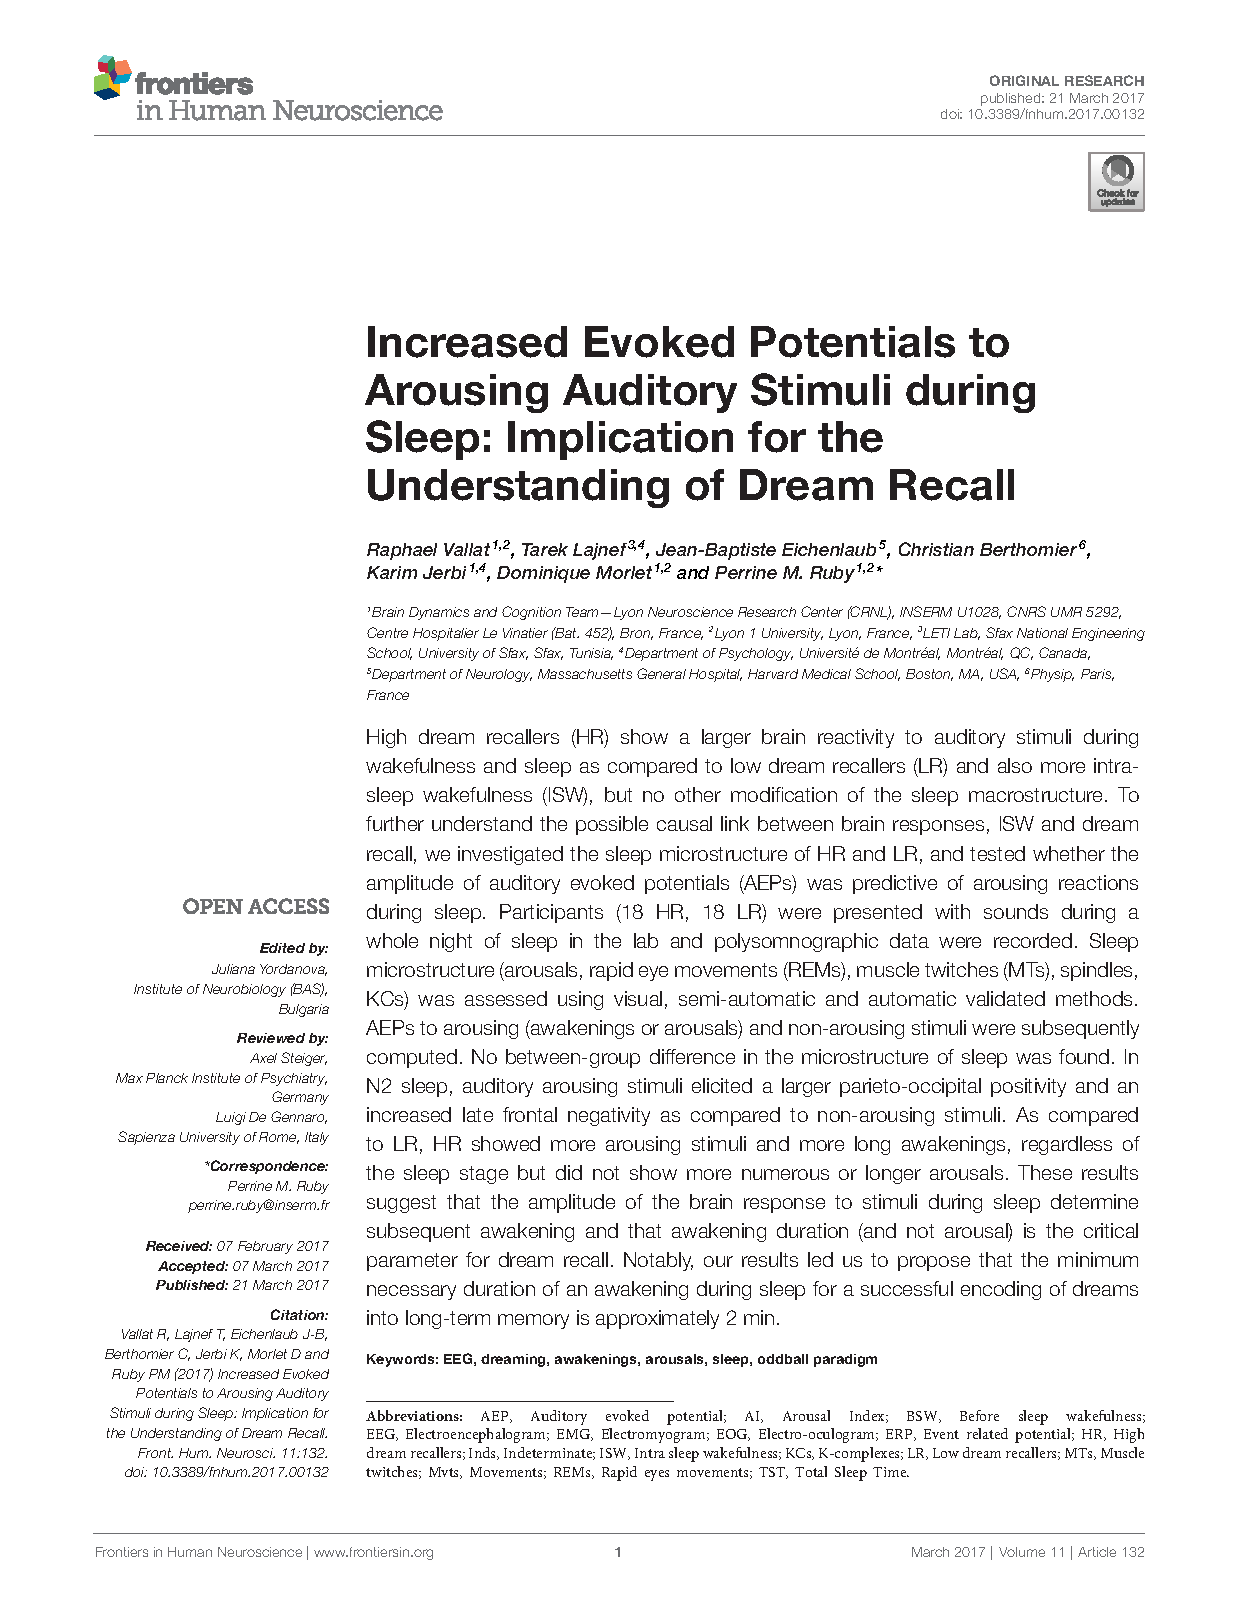
\includepdf[pages=-, pagecommand={\thispagestyle{plain}}]{Articles/Vallat_2017_FHN.pdf}

\cleardoublepage

\subsection*{Supplementary materials}
\label{res:arousal:supp}
\vspace*{1cm}

\begin{figure}[htbp]
	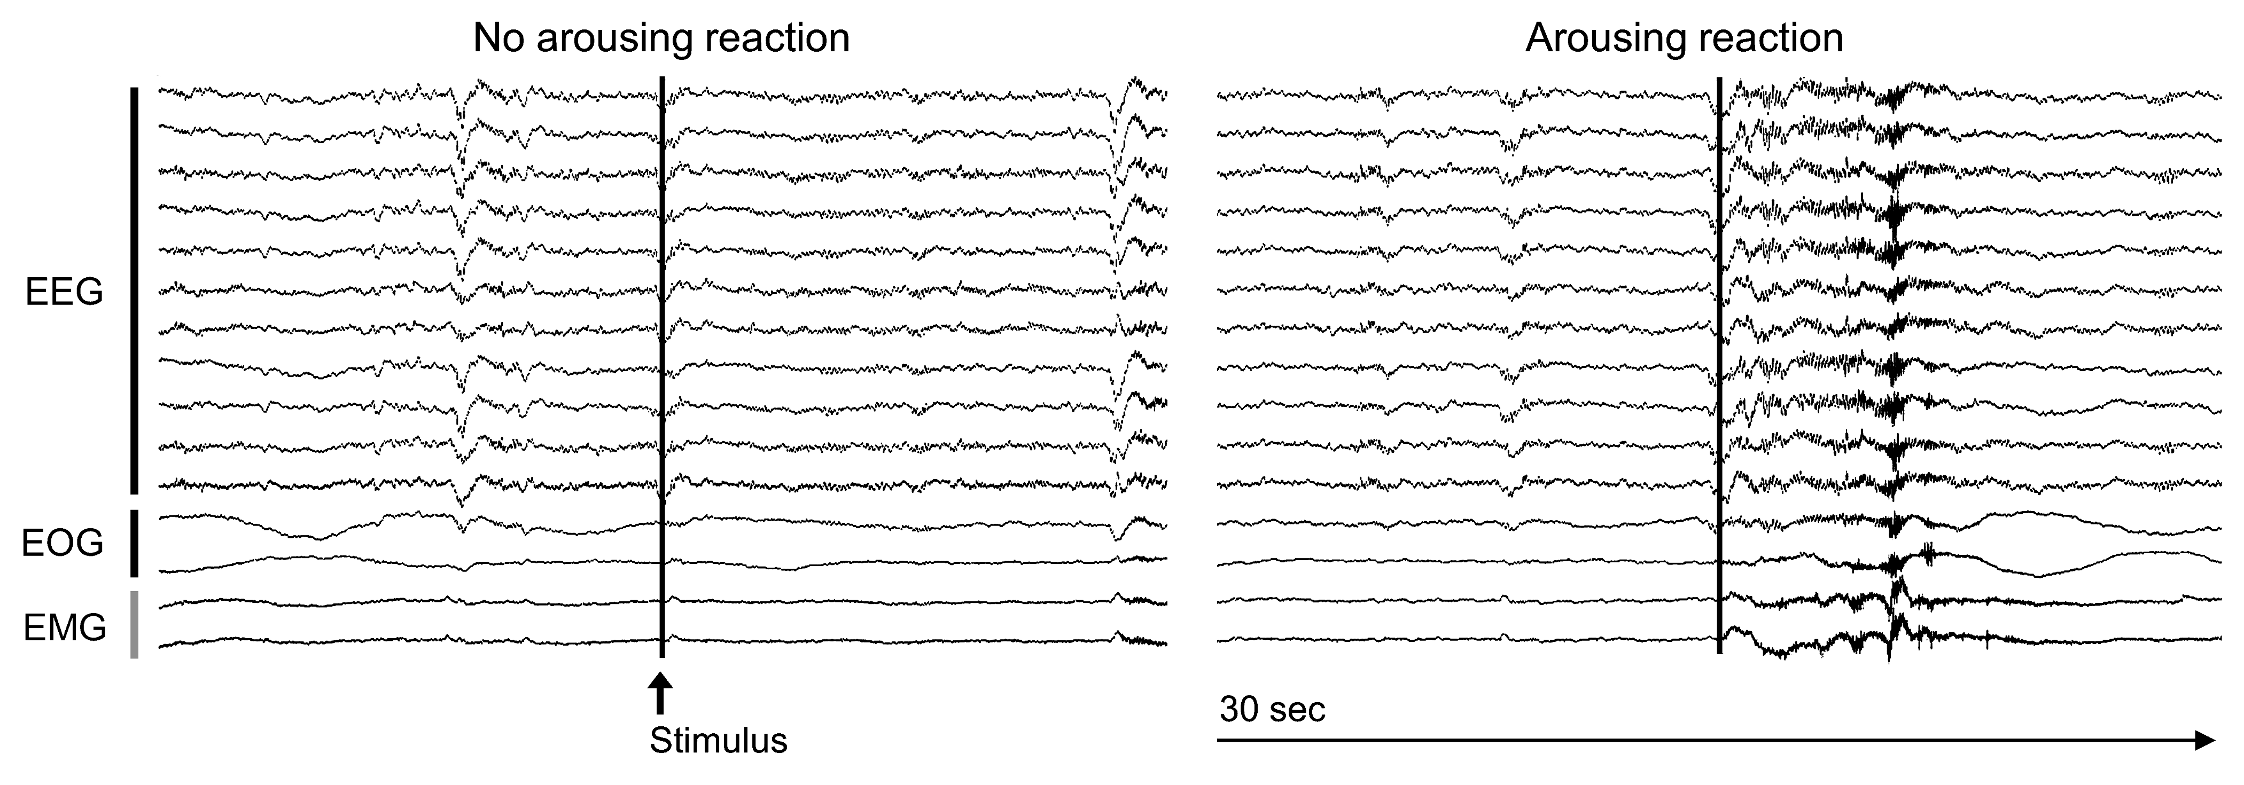
\includegraphics[width=\textwidth]{Fig/Results/Arousals/S1_Fig.png}
	\caption*{\textbf{S1 Fig.} Examples of arousing and non-arousing reactions to auditory stimuli in N2 sleep.}
\end{figure}

\vspace*{3cm}

\begin{figure}[htbp]
	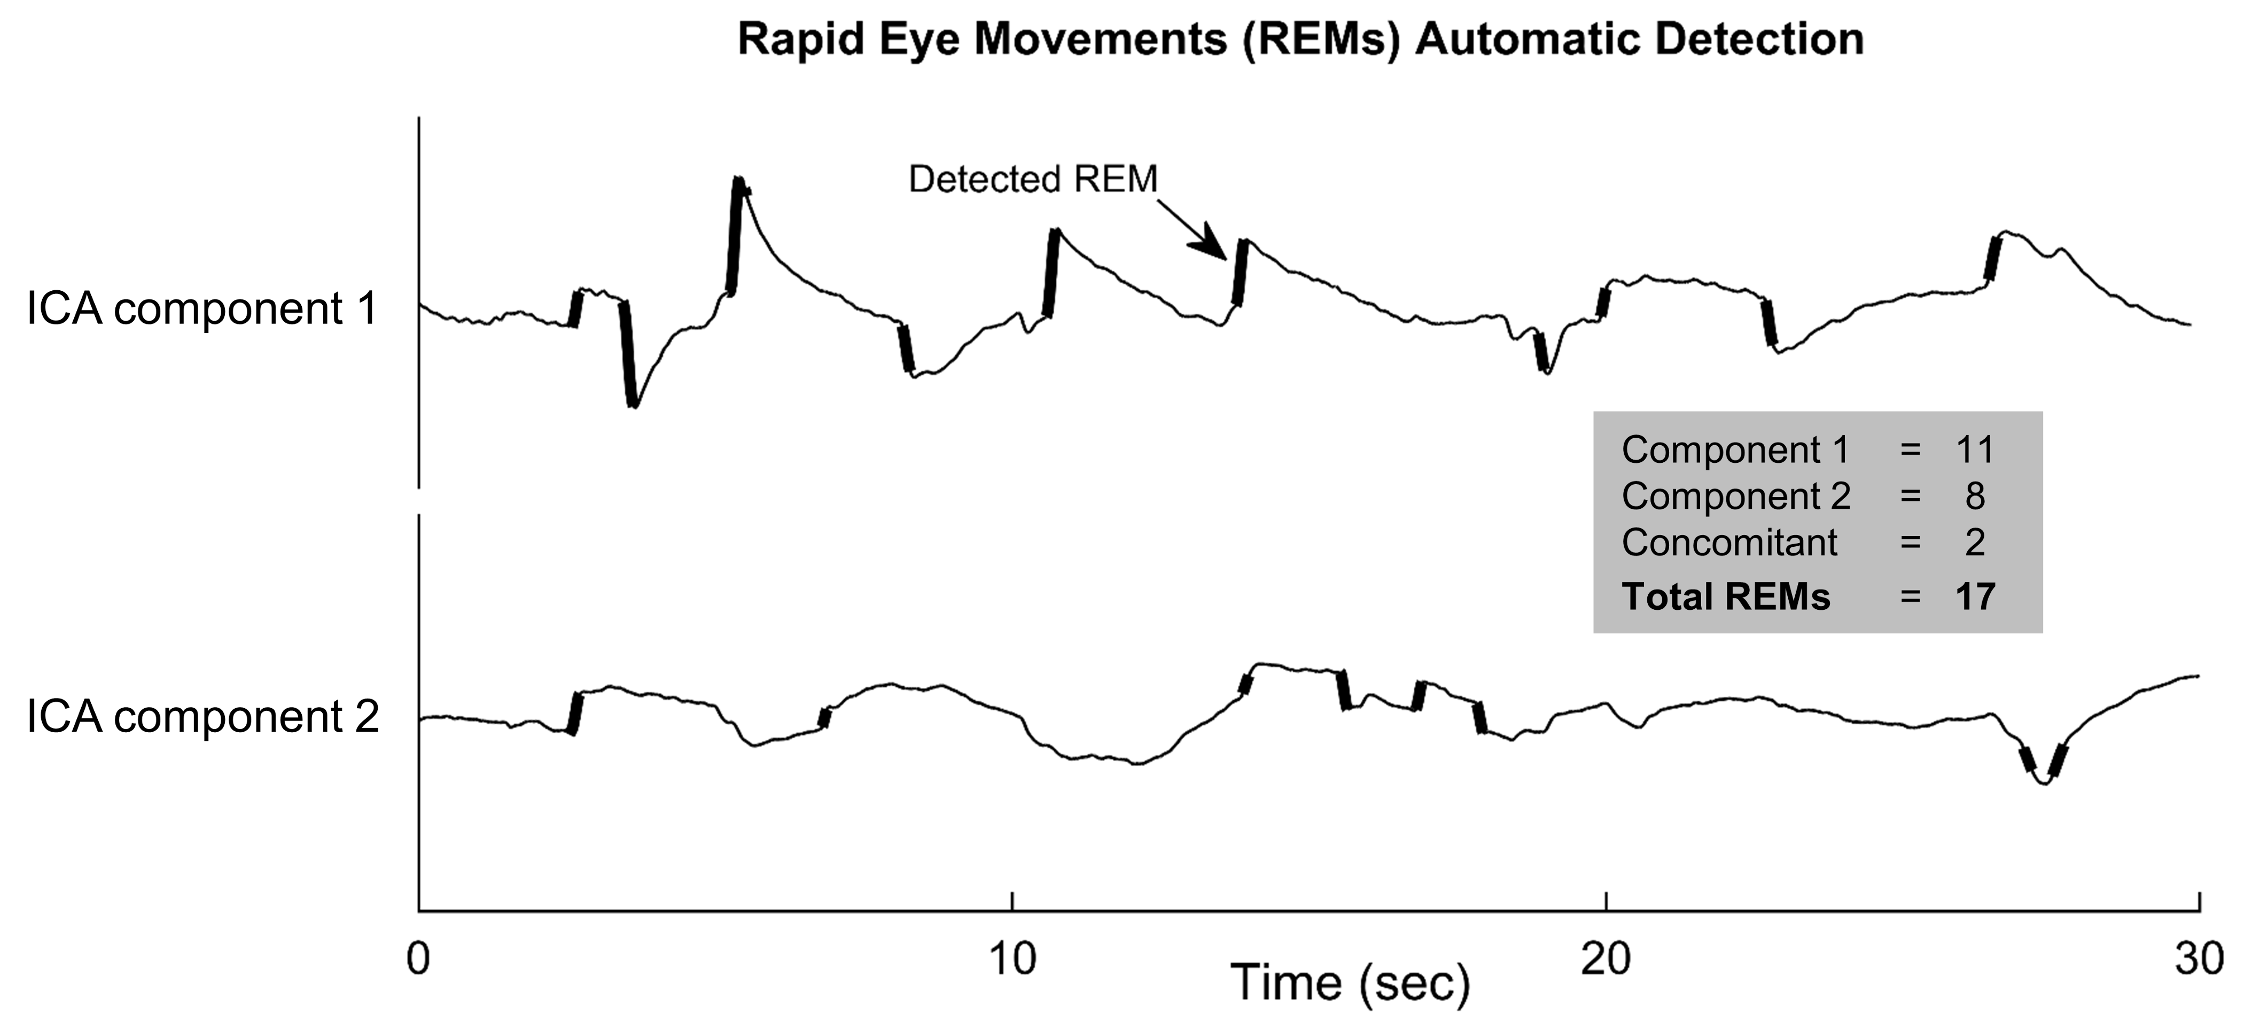
\includegraphics[width=\textwidth]{Fig/Results/Arousals/S2_Fig.png}
	\caption*{\textbf{S2 Fig.} Example of automatic detection of rapid eye movements (REMs) in REM sleep. }
\end{figure}

\begin{figure}[htbp]
	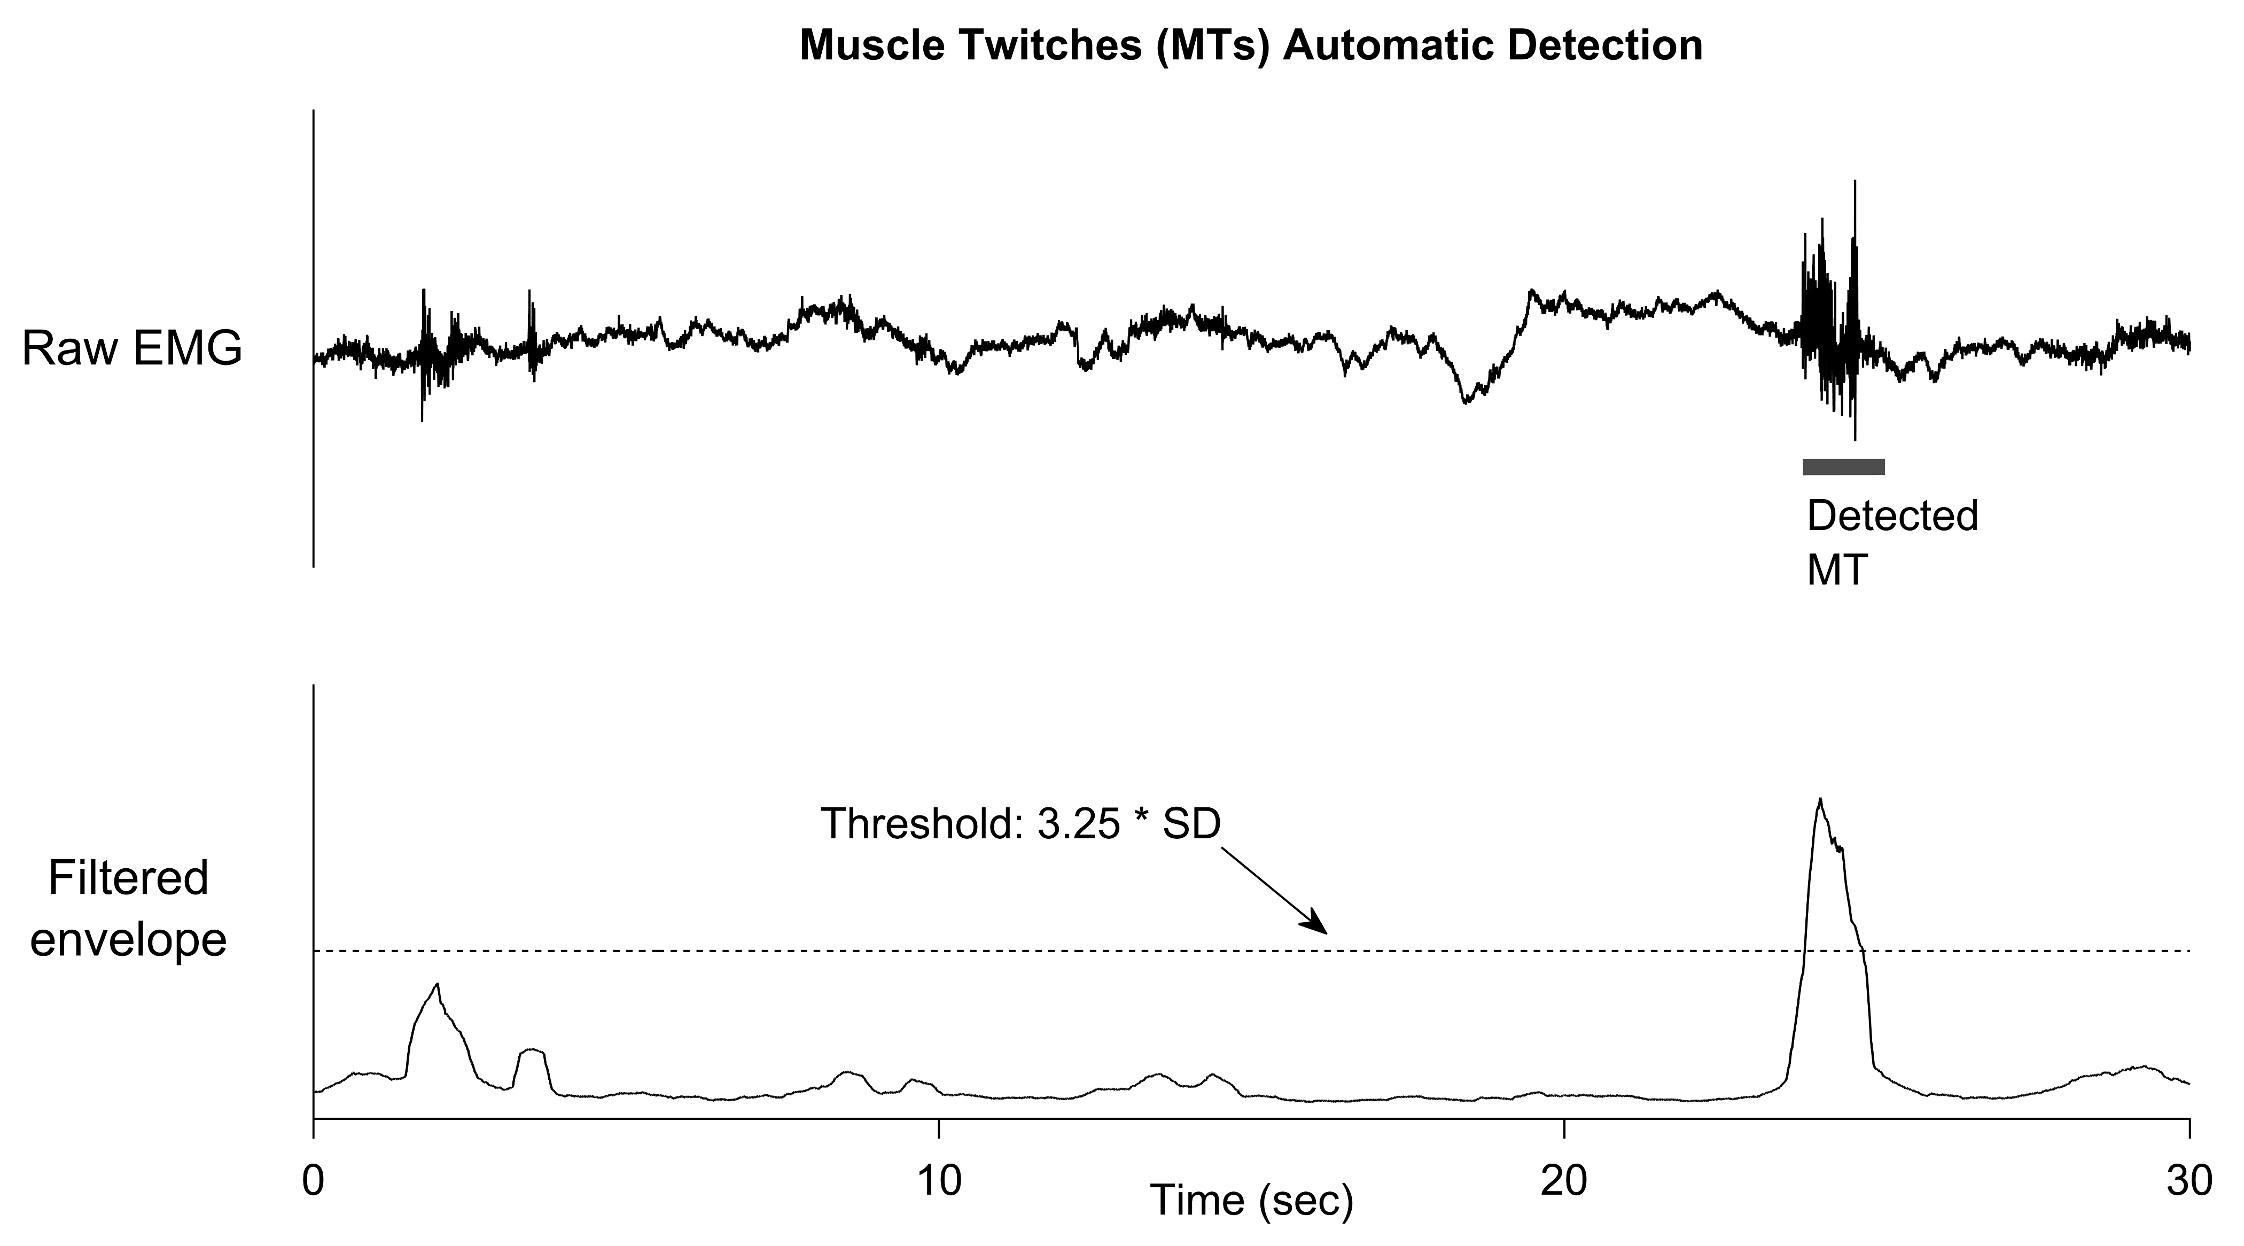
\includegraphics[width=\textwidth]{Fig/Results/Arousals/S3_Fig.png}
	\caption*{\textbf{S3 Fig.} Example of automatic detection of muscle twitches (MTs). Top: Raw EMG signal. Bottom: Smoothed and filtered Hilbert envelope of raw EMG signal. }
\end{figure}

\begin{table}[htb]
    \caption*{\textbf{S1 Table.} Mean ± S.E.M of supplementary macro-structural parameters in High and Low dream recallers, with sleep onset defined as the first page of N1. Last column represents standard values. One-way and two-way ANOVA for independent samples (High-recallers versus Low-recallers) are presented: p<.05*, p<.01**.}
    \resizebox{\textwidth}{!}{%
    \begin{tabularx}{\textwidth}{Xlll}
    \toprule
    Sleep parameters               & High-recallers & Low-recallers & Standard \\ \midrule
    Awakenings, no.                & 19.7 ± 2.2     & 16.3 ± 4.1    & 9.6      \\
    Awakenings, duration (min)     & 1.9 ± 0.2 **   & 1.1 ± 0.1     & 1.4      \\
    Awakenings Index, no. per hour & 3.6 ± 0.5      & 2.8 ± 0.7     & 4.2      \\
    N1                             & 26.5 ± 3.9     & 33.6 ± 4.9    &          \\
    N2                             & 3.4 ± 0.7      & 1.9 ± 0.8     &          \\
    N3                             & 1.0 ± 0.2      & 1.1 ± 0.3     &          \\
    REM                            & 3.6 ± 1.5      & 1.0 ± 0.3     &          \\
    Awakenings duration (\%)       &                &               &          \\
    0-1 min                        & 63.3 ± 3.5 **  & 80.3 ± 3.3    & 87       \\
    1-5 min                        & 28.9 ± 2.5 *   & 18.1 ± 3.2    & 11       \\
    5-30 min                       & 7.8 ± 2.0 **   & 1.6 ± 0.7     & 3        \\ \bottomrule
    \end{tabularx}%
    }
\end{table}
